\section{System Architecture}

Antidote has a plug-in based architecture. So, it was developed a Castalia plugin to support communication between Antidote Stack and Castalia Modules. As the Antidote Library was developed to work with real devices, modifications have been made to the library in reason to work in Castalia Simulator. Communication, encoders, agent and manager are some Antidote's modules changed.

\subsection{Castalia Plugin}

Antidote itself is portable and use ANSI C language to create a standard and clean library. But providing communication between Antidote and others systems, like Castalia, is plug-in dependent. So the dependence of Antidote is just in communication plug-ins.

The proposed plug-in allows Castalia and Antidote talks with each other through \textit{external variables}. Inside Castalia Simulator we can call any function from Antidote Library therefore we can retrieve any information from Antidote library. The problem is to transmit the data from Castalia to Antidote Library. To solve this, we first use external variables to make the data exchange between Castalia and Castalia plug-in module. Then, to obtain the data from Castalia plug-in module, Antidote uses pointers to Plug-in Module functions. That's why we need a plug-in to mediate the communication. 

There are a set of callback functions in Castalia plug-in module that is passed to Antidote during the initialization process of agents. These callback functions are passed to communication module as pointers to functions. This way whenever the communication module needs to retrieve or send a message it just trigger the correspondent callback function. The task of these callback functions is to receive and send messages as also initialize and finalize a agent network.

The Fig.~\ref{fig:CastaliaPlugin} is a representation of the three modules. The arriving messages is copied to an \textit{external variable} in Castalia Simulator Module - the external variable is visible to the both modules Castalia Simulator and Castalia Plugin. Since the communication module in Antidote own pointers to the Castalia Plug-ins functions, it finally can retrieve the messages.

\begin{figure}[htbp]
\centerline{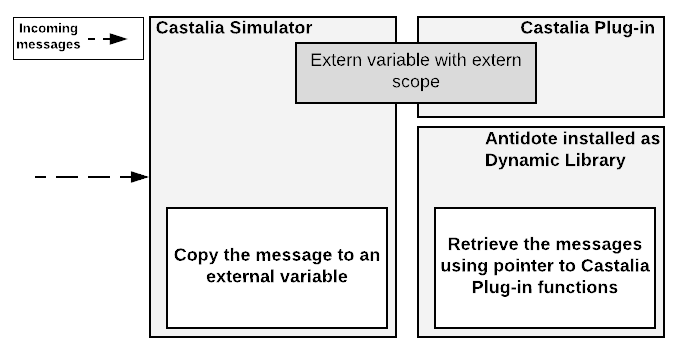
\includegraphics[scale=0.35]{figures/castaliaPlugin.png}}
\caption{How Antidote Library gets the messages from Castalia Simulator.}
\label{fig:CastaliaPlugin}
\end{figure}

\subsection{Changes in communication module}

The Communication module is one of the most important modules in the Antidote. The start, the finalization, transmissions, machine state phases of all nodes are controlled by this module. In a real scenario, each device has your own communication module, running your own copy of the code. So, in one-machine simulation it is a bit different. Only one communication module has to handle with all nodes, since the Antidote Library is installed in the operating system as a dynamic library.

To ensure the proper operation of communication module, the \textit{node id} is required in each method call, this way we know what node we are working with and apply the action just to that node, never affecting another node. For example, if a node transits from unassociated state to associating machine state, without the proposed modification, this action would affect all nodes even those who should not change their machine state.

The Fig.~\ref{fig:communicationModuleCastalia} illustrates the system modifications. In every function in Communication module we insert the \textit{node id} new parameter. This way the communication module always knows the node in question. The arrows in Fig.~\ref{fig:communicationModuleCastalia} represents functions calls.

\begin{figure}[htbp]
\centerline{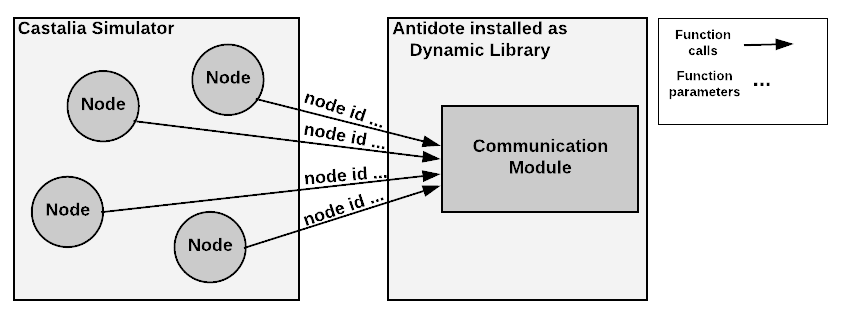
\includegraphics[scale=0.31]{figures/communicationModule.png}}
\caption{Communication module handling several nodes. Each arrow represents a function being called from Communication Module.}
\label{fig:communicationModuleCastalia}
\end{figure}

\subsection{Others modifications}

Others modules like Agent, Manager and Encoders were altered too to smooth operation of Antidote in Castalia. Finalization functions of Agent module were transferred to Manager module for the sake of simplicity and the \textit{node id} were add to the parameters of Agent and Manager modules.

In Encoder module some function were created to interpret the data received. To some devices like Electrocardiography the 11073 standard recommends to convert the measurement data to scaled values before send it. It's useful to send absolute values like $-0.060$  which would require many bytes to be sent. When converted, the number $-0.060$ become $388$, a scaled value which require just two byte to be represented.

Within a Manager, the conversion from scaled to absolute values is given by the expression $Y = M \times X + B$ where:
\begin{align*}
    Y &= \text{the converted absolute value}\\
    M &= \frac{(\text{upper absolute value} - \text{lower absolute value})}{(\text{upper scaled value} - \text{lower scaled value})}\\
    B &= \text{upper absolute value} - (M \times \text{upper scaled value})\\
    X &= \text{the scaled value}
\end{align*}

Within an Agent, the conversion from absolute values to scaled values is given by the expression $X = \frac{(R - B)}{M}$ where:
\begin{align*}
    R &= \text{actual measured value}
\end{align*}

\subsection{Castalia Application}